\documentclass[times, utf8, seminar]{fit}

\usepackage{listings}
\usepackage{longtable}
\usepackage{xcolor}
\usepackage{float}
\usepackage{enumitem}
\usepackage{hyperref}
\usepackage{enumerate}
\usepackage{graphicx}
\usepackage{etoolbox}
\usepackage{datetime}
\usepackage{needspace}
\usepackage{titlesec}

\begin{document}
\widowpenalty=300
\clubpenalty=300
\setlength{\parindent}{0pt}

\lstset{
  language=bash,
  backgroundcolor=\color{gray!25},
  basicstyle=\ttfamily \footnotesize,
  breaklines=true,
  prebreak=\raisebox{0ex}[0ex][0ex] {\ensuremath{\hookleftarrow}},
  columns=fullflexible,
  keywords={},
  mathescape=false
}

\title{Agilni \emph{software development}\newline \emph{Programer kao korisnik}}


% http://en.wikipedia.org/wiki/System_console
% http://en.wikipedia.org/wiki/Computer_terminal


% A terminal emulator, terminal application, term, or tty for short, is a program that emulates a video terminal within some other display architecture. Though typically synonymous with a command line shell or text terminal, the term terminal covers all remote terminals, including graphical interfaces. A terminal emulator inside a graphical user interface is often called a terminal window.


% programerski kalkulator

% http://stackoverflow.com/questions/84421/converting-an-integer-to-a-hexadecimal-string-in-ruby
% irb> "%x" % (0x0FF + 0x0EE) 
% => "1ed" 


\author{Ernad Husremović}
\brindex{DL 2792}
\verzija {0.1.0}
\mentor{mr. Adil Joldić}

\maketitle

\tableofcontents

%\listoftables
%\listoffigures
\newpage

% abstract begin
%\begin{abstract}
%
%To be done 
%
%\keywords{open source software, OSS, Bosna i Hercegovina}
%\end{abstract}

% abstract end

\chapter{Uvod}

\emph{Human-computer interaction (HCI)}\footnote{Interakcija čovjek-računar} pročava zakonitosti interakcije čovjeka i računara.

Koncept grafičkog interfejsa (GUI), miš (mouse), ekran osjetljiv na dodir (eng. touch screen) očiti rezultati izučavanja HCI-a.

\section{Kategorizacije korisnika}

Različite skupine korisnika imaju različite zahtjeve i potrebe u kontekstu HCI-a. 

Tako malo dijete prepoznaje slike, ali ne razumije slova. Starijim i slabovidnim osobama odgovaraju veći prikazi. \enb{"Touch screen"} je intuitivan ulazno-izlazni uređaj, čak i za dijete od tri-četiri godine. Tastatura to nije. Pripadnost određenoj starosnoj skupini određuje moguće načine interakcije sa računarom.

Sljedeća bitna kategorizacija korisnika određena je poslovima koje korisnik obavlja na računaru. 

U uputstvima za korištenje software-a se ova karakteristika jednostavno naziva "korisnička ciljna grupa". Softverska rješenja su često složeni proizvodi, namjenjeni za \emph{više ciljnih grupa} odjednom. Tako ćemo u uputstvima često naći sljedeće:
\begin{itemize}
  \item Pogodno za korisnika "početnog nivoa".
  \item Ova opcija je namjenjena isključivo naprednim korisnicima.
  \item Pristup dozvoljen samo Administratoru\footnote{Administrator sistema - stručna osoba zadužena za funkcionisanje sistema} sistema
\end{itemize}

\section{Produktivnost korisnika}

Dobro softverskog rješenje je bez dvojbe mora biti sa stanovišta korisnika \emph{produktivno}. Ono mora pomoći da se posao koji se obavlja brže i efikasnije sa tim software-om nego li bez nega.

Produktivnost pretpostavlja niz stavki koje je potrebno zadovoljiti:
\begin{itemize}
  \item tačnost - \emph{software} treba obezbjediti korsniku tačne rezultate
  \item fleksibilnost - software treba predvidjeti sve bitne varijante korištenja sa stanovišta korisnika
  \item robusnost - u slučaju problema i grešaka, gubici i zastoji korisnika trebaju biti minimalni
\end{itemize}


\section{Potrebni period učenja software-a (eng. \emph{Sofware Learning Curve}}

Poduktivnost "ne leži" samo u implementaciji softverskog rješenja. Produktivnost se postiže dobrim poznavanjem software-a od strane korisnika. Time dolazimo do još jedne bitne karakteristike software-a: Potrebni period učenja - \emph{Learning curve}.\footnote{Doslovni prevod na bio bi bosanski "krivulja učenja"}

Cilj je svakako da taj period bude što manji. Ono što je veoma bitno, jeste postizanje napretka u početnom periodu učenja. Ukoliko korisnik ne stekne osjećaj postignuća u početnom periodu, postoji velika mogućnost da će odustati od ponuđenog, posebno ako su mu na raspolaganju alternativna rješenja.

\section{Navike korisnika}

Kada se korisnik osposobi za korištenje određenog softverskog rješenja, on prirodom stvari stiče navike. Prosječan korisnik mnoge stvari obavlja po \emph{inerciji}. Čak i kada drugi korisnici postižu bolje rezultate, čak i kada su troškovi prelaska na druga rješenja minimalni, prosječan korisnik nije sklon promjenama software-a na koji je navikao. Stoga je, posebno u poslovnim primjenama, odabir odgovarajućeg rješenja veoma bitan korak.

\section{Kategorizacije programera}

Fokusirajmo se sada na programere kao posebnu ciljnu grupu. Sa stanovišta primarnih zaduženja, u domenu izrade poslovnih softverskih rješenja, adekvatna sljedeća podjela:

\begin{itemize}
  \item aplikativni programer - zadužen za održavanje i realizaciju standarndih funkcija softverskog rješenja, usmjerenih ka krajnjem korsniku 
  \item programer baznih funkcija (\emph{"core Libraries"}) - zadužen za niže nivoe arhitekture software-a
\end{itemize}

Aplikativni programer je tako zadužen za izradu novog izvještaja "Pregled dugovanja kupaca koji su prekoračili rok dospijeća obaveze",  dok je "core" programer zadužen za realizaciju opcije "Razmjene podataka između prodavnica i centralne lokacije".  

Možemo nastaviti u dubinu sa ovom podjelom po sljedećim karakteristikama. Prema nivou vještina i iskustva: 
\begin{itemize}
  \item početnik - junior programer
  \item iskusni - senior programer
\end{itemize}

Softverska rješenja su složeni sistemi. Pojedine komponente traže dodatnu ekspertizu - specijalizaciju programera:
\begin{itemize}
  \item database programer
  \item programer korisničkog interfejsa (UI)
  \item programer web rješenja
     \begin{itemize}
          \item back-end
          \item front-end
      \end{itemize}
\end{itemize}

Ako posmatramo softverski projekat i njegov životni ciklus u cjelini, pored razvoja imamo i operacije podrške i instalacije\footnote{Često su u sve ove operacije programeri u većoj ili manjoj mjeri uključeni. Može se reći da je to čak pravilo ununtar manjih razvojnih timova}: 
\begin{itemize}
   \item poslovi podrške
   \item poslovi sistemske administracije
   \item poslovi razvoja i dizajna
\end{itemize}

\section{Agilni software development}

Agilni pristup se bazira na multi-funkcionalnim. Članovi takvog tima su posljedično generalisti\citep[str. 19]{agilesamurai}:

\begin{quote}
\emph{Kada formirate vaš tim, trebate generaliste, osobe koje nemaju problem raditi široki spektar stvari. Za programere, to znači naći osobe koje su sposobne raditi sa kompletnim tehnološkim stekom projekta (ne samo front-end ili back-end). Za testere i analiste, to znači osobe koje su spremne obaviti kako uobičajena testiranja, tako i detaljne analize korisničkih zahtjeva.}
\end{quote}

\section{Produktivnost programera}

U predhodnih 20 godina, povećanje produktivnosti se pokušalo postići na mnoge načine. Izdvojimo načine koji su posebno interesantni:

\begin{itemize}
  \item Izradom visoko sofisticiranih CASE\footnote{\url{http://en.wikipedia.org/wiki/Computer-aided_software_engineering#Tools}} alata
  \item Integrirana razvojna okruženja (IDE)\footnote{\url{http://en.wikipedia.org/wiki/Integrated_development_environment}} 
\end{itemize}

\subsection{CASE alati}

CASE alati su bili posebno popularan koncept kraja 80-ih i 90-ih godina (do ekspanzije interneta). CASE alati su pred sebe postavili iznimno ambiciozan cilj: napraviti okruženje koje će automatizirati kompletan životni ciklus razvoja software-a. Pri tome, zamišljeno je da se sam razvoj aplikacije realizira na visokom stepenu apstrakcije. Da bi se to postiglo, dizajneri CASE alata su trebali obezbjediti "kostur" aplikacije koji bi aplikativni programeri koristili kao polaznu tačku. Međutim, na kraju se pokazalo da tom konceptu nedostaje \emph{fleksibilnost}. Koliko god dobar dobro dizajniran CASE alati nisu mogli obuhvatiti sve moguće scenarije razvoja aplikacija. U konačnici, CASE alat može pružiti visoki stepen produktivnosti u početku razvoja, ali se ta prednost brzo "istopi" u kasnijim fazama razvoja aplikacija. 

Može se reži da su CASE alati pokušali pokušali kompleksne, kreativne faze razvoja software-a što više prebaciti u same CASE proizvode. Eksperti - dizajneri CASE alata prave ''kostur'' (eng. application skeleton), dok programeri - korisnici CASE-a realiziraju po tom već ustavnovljenom šablonu programska rješenja za krajnjeg korisnika. Zamisao je da se time posao aplikativnog programera svodi na manje više rutinski, dosta jednostavan posao.

Međutim, rezultat su bila rješenja koja nisu mogla zadovoljiti potrebama korisnika. CASE alati se jednostavno nisu mogli obuhvatiti svu raznolikost zahtjeva i potreba korisnika u realnom okruženju.

Drugi bitan faktor neuspjeha CASE koncepta je internet era, odnosno potreba za www\footnote{\url{http://hr.wikipedia.org/wiki/World_Wide_Web}} rješenjima. CASE alati nisu bili platforma za razvoj web rješenja\footnote{Web standardi su bili u povoju. Arhitektura web rješenja je u početku bila nejasna, fagmentacija web browsera velika}.

\subsection{IDE alati}

IDE alati su, za razliku od CASE alata ipak našli svoje mjesto u standardnom developerskom setu alata. Tu međutim treba imati na umu na opcije koje su u početku smatrane ključnim, marginalizirane po sličnom principu kao u slučaju CASE-a alata. Dobar primjer je funkcija Vizuelnog dizajnera formi (eng. Visual Forms Designer). Prve generacije IDE alata su ovu funkciju stavljale na vrh liste funkcija. Pokazalo se međutim da funkcije vizuelnog dizajniranja, čim aplikacija dosegne određeni nivo kompleksnosti, zna postati neadekvatna. Kada se to desi, vizuelni mod se napušta, i programer (ponovo) piše forme direktno u kodu. Takođe, ''Visual Forms'' alati do sada nisu postigli veliku primjenu na području razvoja web aplikacija, što je konceptu ''vizuelnog programiranja'' dodatno umanjilo na bitnosti. 

IDE okruženja su zato fokus razvoja usmjerili na produktivnost programera unutar \emph{source code} editora. Ključne opcije postaju funkcije koje asistiraju programeru:
\begin{itemize}
  \item automatsko kompletiranje imena funkcija, varijabli, klasa\footnote{Microsoftova implementacija \url{http://en.wikipedia.org/wiki/IntelliSense}}
  \item sugestije i pomoć programeru prilikom pisanja izvornog koda 
     \begin{itemize}
        \item pomoć pri formatiranju k\^oda - \eng{autoindent}
        \item provjera sintakse - \emph{syntax checking}
      \end{itemize}
  \item integrirano debugiranje
\end{itemize}

\section{Programski jezici}

Expanzija zahtjeva za web i mobilnim rješenjima je rezultirala pravom ''invazijom'' programskih jezika. 

\subsection{Java, univerzalni programski jezik}

''Java''\footnote{\url{http://en.wikipedia.org/wiki/Java_(programming_language)}} nije ostvarila očekivanja univerzalnog programskog jezika. Posebno su se pokazali nedostatnim: 
\begin{itemize}
  \item java na strani web klijenta (java web plugin sistem)
  \item kompleksnost java serverskog steka J2EE\footnote{\url{http://radio-weblogs.com/0135826/2004/03/17.html}} 
\end{itemize}

U posljednjim implementacijama J2EE\footnote{\url{http://en.wikipedia.org/wiki/Java_Platform,_Enterprise_Edition}} su napravljeni značajni pomaci. Međutim, veliki broj developera je prihvatio alternativne tehnologije i programske jezike.

\subsection{Dinamički programski jezici}

Nova generacija developera, posebno u domenu razvoja web aplikacija, usvaja dinamičke programske jezike\footnote{\url{http://en.wikipedia.org/wiki/Dynamic_programming_language}}. 
 
Jedan od ključnih faktora tog trenda je značajno skraćen \emph{Learning curve} u odnosu na konvencionalne platforme (J2EE, .NET).

\subsection{Javascript, \emph{''Lingua franca''}} web-a\footnote{\url{http://en.wikipedia.org/wiki/JavaScript}}

Ekspanzija web-a je dovela do neslućene ekspanzije ``Javascript`` programskog jezika\footnote{\url{http://en.wikipedia.org/wiki/JavaScript}}. Primarno zamišljen kao programski jezik \emph{web browsera}, javascript se počinje primjenjivati i van browsera:
\begin{itemize}
  \item mobilni klijent - appcelerator titanium\footnote{\url{http://www.appcelerator.com/platform/titanium-sdk}}
  \item \emph{server-side} - node.js\footnote{\url{http://nodejs.org}}
  \item \emph{database stored procedure} - plv8\footnote{\url{http://code.google.com/p/plv8js/wiki/PLV8}}
\end{itemize} 

\chapter{Developerski \emph{toolbox} nove generacije developera}

Dinamički programski jezici (php, python, ruby, javascript) su generirali potrebe za razvojem nove generacije programerskih alata. 

Tu se pojavio značajan problem. Niz funkcija koje je relativno jednostavno implementirati kod \emph{strong-type}\footnote{\emph{http://en.wikipedia.org/wiki/Strong_typing}} programskih jezika\footnote{Dobar je primjer \emph{autocomplete} funkcija IDE-a}, je teško realizovati kod dinamičkih jezika.


Nova generacija developera iz temelja mijenja svoj toolbox. Kako konvencionalni IDE alati manjkaju naprednom podrškom dinamičkim jezicima, oni ponovo istražuju alternativna rješenja.

\section{Povratak u prošlost - komandna linija i programerski editor}

Njihov odabir je krajnje interesantan. Oni u svakodnevnom radu intenzivno koriste ''starinske'' alate:
\begin{itemize}
  \item Umjesto IDE okruženja, koriste programerske editore\footnote{\url{http://net.tutsplus.com/tag/code-editors/}} vi, emacs\footnote{Oni konvencinalniji Notepad++, TextMate, jEdit}
  \item intenizvno koriste terminal i komandnu liniju\footnote{\url{http://en.wikipedia.org/wiki/Strong_typing}} 
\end{itemize}

\section{TDD umjesto \emph{debugera}}

Podrške interaktivnom debugiranju dinamičkih jezika je, posebno u početku, bila na niskom nivou. Taj nedostatak je značajno uticao na pojavu nove paradigme programiranja: \emph{Test driven development} - (TDD)\footnote{\url{http://en.wikipedia.org/wiki/Test-driven_development}}.

TDD se brzo pokazao kao pozitivna programerska praksa koja utiče na povećanje kvaliteta izvornog k\^oda neovisno od nivoa podrške debugiranju. 

\section{Dolazeća generacija programerskih alata}

\emph{''Javascript everywhere''} princip širi se i na područje programerskih alata:
\begin{itemize}
   \item \emph{Adobe Brackets code editor} - \url{http://brackets.io}
   \item \emph{online} - alati u \emph{cloud}-u:
   \begin{itemize}
     \item \emph{CloudIDE} - \url{https://c9.io}
     \item \emph{Github code snippets} - \url{https://gist.github.com}
   \end{itemize}
\end{itemize}

Video nettuts+ ''A Peek At Brackets''\footnote{\url{http://www.youtube.com/watch?v=HZkrlX7jJcg}} ukazuje na inovativni pristup produktivnom pisanju Javascript/HTML/CSS k\^oda.

\begin{figure}[H]
\centering
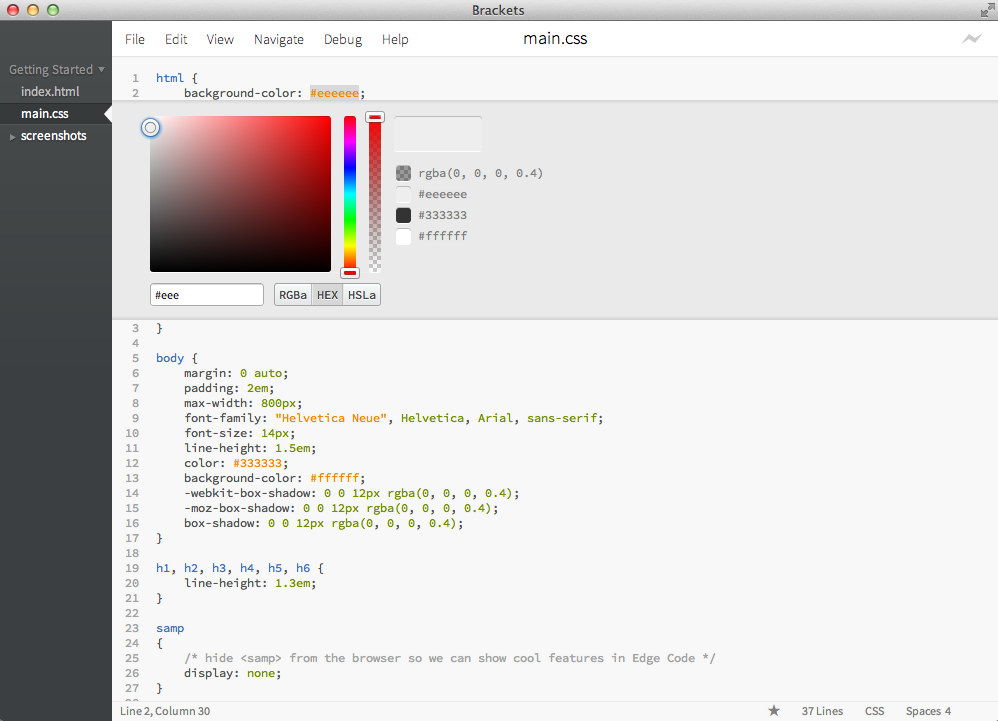
\includegraphics[width=15cm]{img/brackets_color_edit.png}
\caption{Brackets code editor - \emph{quick edit} ''color'' elementa}
\end{figure}

Programerski alati u \emph{cloud}-u je drugi značajan trend u ovoj oblasti. Socijalni aspekt \emph{online} alata - pojednostavljena komunikacija između developera su bitan katalizator ovih promjena.

\chapter{Komandna linija}

''Novi developer'' svakodnevno koristi terminal\footnote{\url{http://en.wikipedia.org/wiki/Terminal_emulator}} i komandnu liniju. U ovom poglavlju ćemo prikazati najbitnije načine korištenja \emph{command-line} alata.

\section{\emph{Command-line} interfejs sa stanovišta HCI-a}

Prednosti \emph{Command-line} interfejsa\footnote{\url{http://www.cs.man.ac.uk/~seanb/teaching/COMP10092/COMP10092-HCI.pdf}}:
\begin{itemize}
 \item brz i moćan za iskusne korisnike
 \item minimalna količina tipkanja (miš se ne koristi)
 \item može se koristiti u kombinaciji sa drugim korisničkim interfejsima
\end{itemize}

Nedostaci:
\begin{itemize}
\item izvršenje komandi sa malo ili bez pitanja korisnika
\item traži dobro poznavanje sistema i programa
\item bazira se na sjećanju - memorisanju komandi i sintakse
\item težak za učenje
\item sklon greškama
\end{itemize}

%Menu:
%
%Advantages
%Users don't have to memorize complex commands
%Structured navigation benefits novices and casual users
%Can shorten user learning time and effort
%Supports recognition memory
%
%
%Disadvantages
% May not be appropriate or efficient for some users and tasks
%Can force user through many levels of menus
%Users may get lost in menu hierarchies
%Menu terms and names may not be meaningful to users
%Use of modes forces users to follow the system's path
%
%

\section{\emph{Unix Pipe}}

\emph{Unix Pipeline}\footnote{\url{http://en.wikipedia.org/wiki/Pipeline_(Unix)}} je jednostavan, ali nadasve moćan koncept kreiranja složenih komandi preusmjeravanjem izlaza predhodne u ulaz naredne komande.

\begin{figure}[H]
\$ \verb+ps ax | grep MacVim | grep -v grep+
\begin{lstlisting}
  585   ??  S      1:13.89 /Applications/MacVim.app/Contents/MacOS/MacVim -psn_0_249917
86785   ??  Ss     0:00.23 /Applications/MacVim.app/Contents/MacOS/Vim -g -f --mmwaitforack
\end{lstlisting}

\caption{Pregled svih ''MacVim'' trenutno aktivnih procesa}
\end{figure}



\section{\emph{Read-eval-print-loop} (REPL)}

Dinamički jezik redovno sadrži REPL\footnote{\url{http://en.wikipedia.org/wiki/Read–eval–print_loop}} režim.
REPL omogućava interaktivni unos komandi dinamičkog programskog jezika.

\subsection{Programerski kalkulator bez limita - \emph{irb}}

Ruby\footnote{\url{http://www.ruby-lang.org}} REPL konzola naziva se \verb+irb+. 


\begin{figure}[H]
\$ \verb+irb+

\begin{lstlisting}
$ irb
1.9.3p286 :001 > 228 % 15 # cjelobrojni ostatak
 => 3 
1.9.3p286 :002 > 2**3 # stepenovanje
 => 8 
1.9.3p286 :003 > a = 2**3 + 528/5.2
 => 109.53846153846153 
1.9.3p286 :004 > b = Math.sin(0.2) + 2 * Math.cos(0.8)
 => 1.5920827494893923 
1.9.3p286 :005 > a + 2.2 / b
 => 110.92029926059348
\end{lstlisting}

\caption{ruby ''irb'' - kalkulator bez limita}
\end{figure}


% http://lifehacker.com/385929/best-text-editors

% http://sourceforge.net/apps/mediawiki/notepad-plus/index.php?title=Plugin_Central


% vim
% https://github.com/joonty/vdebug
% https://github.com/thoughtbot/vimulator


% http://en.wikipedia.org/wiki/Human_computer_interaction

% Human-omputer Interaction (HCI) involves the study, planning, and design of the interaction between people (users) and computers. It is often regarded as the intersection of computer science, behavioral sciences, design and several other fields of study. The term was popularized by Card, Moran, and Newell in their seminal 1983 book, "The Psychology of Human-Computer Interaction", although the authors first used the term in 1980[1], and the first known use was in 1975[2]. The term connotes that, unlike other tools with only limited uses (such as a hammer, useful for driving nails, but not much else), a computer has many affordances for use and this takes place in an open-ended dialog between the user and the computer.
% Because human–computer interaction studies a human and a machine in conjunction, it draws from supporting knowledge on both the machine and the human side. On the machine side, techniques in computer graphics, operating systems, programming languages, and development environments are relevant. On the human side, communication theory, graphic and industrial design disciplines, linguistics, social sciences, cognitive psychology, and human factors such as computer user satisfaction are relevant. Engineering and design methods are also relevant. Due to the multidisciplinary nature of HCI, people with different backgrounds contribute to its success. HCI is also sometimes referred to as man–machine interaction (MMI) or computer–human interaction (CHI).

% xmodmap i vim http://www.8t8.us/vim/vim.html

% tselect pattern http://stackoverflow.com/questions/4963019/search-for-a-tag

% unite-vim http://www.vim.org/scripts/script.php?script_id=3396

% https://github.com/hernad/neocomplcache

% http://en.wikipedia.org/wiki/Command-line_interface

%A command-line interface (CLI) is a means of interaction with a computer program where the user (or client) issues commands to a program in the form of successive lines of text (command lines).
%The command-line interface evolved from a form of dialog once conducted by humans over teleprinter machines, in which human operators remotely exchanged information, usually one line of text at a time. Early computer systems often used teleprinter machines as the means of interaction with a human operator. The computer became one end of the human-to-human teleprinter model. So instead of a human communicating with another human over a teleprinter, a human communicated with a computer.
%In time, the actual mechanical teleprinter was replaced by a glass tty (keyboard and screen, but emulating the teleprinter), and then by a terminal (where the computer software could address all of the screen, rather than only print successive lines).

%
%\section{Cloud i command line intefejs}

% http://www.h-online.com/open/news/item/Amazon-releases-preview-of-command-line-for-cloud-services-1774374.html

%
%
%\section{Zašto developer voli ''vim'', ''tmux'' i ''konzolu''}
%
%\section{Zašto se pojavio PowerShell ?}
%
%Jer su to ''Windows'' developeri tražli.
%
%Zašto su to tražili ?
%
%Radi automatizacije. GUI alati jesu lagani i intuitivni za rukovanje ali se te operacije ne mogu automatizirati.
%
%Koliko god konzola izgledala anahrona u odnosu na GUI interfejs, oni su uočili šta se na toj konzoli, sa bash i sličnim skriptnim jezicima može postići.
%

%\section{Zašto najnovija verzija titanium okruženja sadrži moćan CLI ?}
%
%Jer su to developeri tražili
%
\section{Zašto nijedan git GUI \emph{shell} obezbjeđuje samo osnovni set komandi}

Git je iznimno fleksibilan, ali i kompleksan alat. GUI alati obezbjeđuju obične, najčešće korištene operacije
\begin{itemize}
 \item init, add
 \item pull
 \item commit
 \item push
 \item log, diff
\end{itemize}

Međutim, pored toga


\begin{lstlisting}
~$ git --help

=>

usage: git [--version] [--exec-path[=<path>]] [--html-path] [--man-path] [--info-path]
           [-p|--paginate|--no-pager] [--no-replace-objects] [--bare]
           [--git-dir=<path>] [--work-tree=<path>] [--namespace=<name>]
           [-c name=value] [--help]
           <command> [<args>]

The most commonly used git commands are:
   add        Add file contents to the index
   bisect     Find by binary search the change that introduced a bug
   branch     List, create, or delete branches
   checkout   Checkout a branch or paths to the working tree
   clone      Clone a repository into a new directory
   commit     Record changes to the repository
   diff       Show changes between commits, commit and working tree, etc
   fetch      Download objects and refs from another repository
   grep       Print lines matching a pattern
   init       Create an empty git repository or reinitialize an existing one
   log        Show commit logs
   merge      Join two or more development histories together
   mv         Move or rename a file, a directory, or a symlink
   pull       Fetch from and merge with another repository or a local branch
   push       Update remote refs along with associated objects
   rebase     Forward-port local commits to the updated upstream head
   reset      Reset current HEAD to the specified state
   rm         Remove files from the working tree and from the index
   show       Show various types of objects
   status     Show the working tree status
   tag        Create, list, delete or verify a tag object signed with GPG

See 'git help <command>' for more information on a specific command.
\end{lstlisting}

Međutim, operacije kao što su ''branch'' i ''tag'', ''merge'' se uobičajeno obavljaju sa komandne linije.
One imaju toliko varijanti i mogućih scenarija realizacije, da je implementacija kroz GUI shell gotovo nemoguća. Čak i kada bi se sve to realiziralo, pitanje konačnog korisničkog iskustva takve implementacije je krajnje diskutabilno.

''GUI''


iranje i tagiranje


\begin{lstlisting}
~$ ps ax | grep tmux

=>

75447   ??  Ss     0:49.87 tmux
76174 s007  S+     0:00.01 tmux a
 3148 s014  S+     0:00.00 grep tmux
\end{lstlisting}

\begin{lstlisting}
~$ ps ax | grep tmux | grep -v grep

=>

75447   ??  Rs     0:49.88 tmux
76174 s007  S+     0:00.01 tmux a
\end{lstlisting}

\begin{lstlisting}
~$ ps ax | grep tmux | grep -v grep | grep -c tmux

=> 2
\end{lstlisting}


Zašto db administrator pored svih ''visual'' alata voli sql konzolu ?


\chapter{Zaključak}

Produktivnost


% -------------------------------------------------
\bibliography{literatura}
\bibliographystyle{fit}

\end{document}
